% axiesproc クラスを利用します
% このクラスは jsarticle に依存し, ひいては pLaTeX2e を要求します
\documentclass{jsaxiesproc}

% 必要に応じ, 適宜パッケージを追加してください.
% usepackage{amsmath}
\usepackage[dvipdfmx]{graphicx,color,hyperref}


% 和文タイトル
\title{
	RAGで最適化した生成AIによるHPCユーザ向けサービスの実現
}

\author{
三上和徳$^{1,a)}$,
中村宜文$^{1,b)}$,
庄司文由$^{1,c)}$
}

\affiliation{
1) 理化学研究所 計算科学研究センター
}

\contactemail{
a)kazunori.mikami@riken.jp,
b)nakamura@riken.jp,
c)shoji@riken.jp
}

% 英文タイトル
\etitle{
	Realization of HPC User Services Using Generative AI Optimized with RAG
}

\eauthor{
Kazunori Mikami$^{1,a)}$,
Yoshifumi Nakamura$^{1,b)}$,
Fumiyoshi Shoji$^{1,c)}$
}

\eaffiliation{
1) RIKEN Center for Computational Science
}



\begin{abstract}
理化学研究所計算科学研究センター(R-CCS)ではスーパーコンピュータ「富岳」のユーザから寄せられる様々な技術的質問や要望へのサポートを行う「富岳サポートサイト」におけるサービスの一環として、2024年度から生成AIによるサービスを加え、ユーザ自身による迅速な自己解決を実現するための取り組みを推進している。
本稿ではR-CCSが生成AIをサービスに採用した経緯、RAGを応用した最適な生成AIサービスの構築、得られた効果などに関して報告を行う。また、同じ生成AI技術を応用してサービスを開始したHPCI利用報告書の閲覧支援サービスについても紹介をする。
\end{abstract}

\begin{document}
\maketitle



\textcolor{red}{
用語確認:生成AIか、単にAIとするか?
}




\section{ユーザをサポートするサービス基盤}
「富岳」の利用にあたって、ユーザは利用手引書の内容を理解した上で各自の課題に取り組むことになるが、特に利用当初は利用方法についての疑問が生じたりエラーへの対処方法を調査することが必要となる局面がしばしば発生することがある。そのような質問や申請を受け付けて対処方法を示す、いわゆるユーザサポートは「富岳」を効果的に利用して成果の創出を後押しする上での重要な役割を担うことになる。
以下に「富岳」ユーザに向けたサポートサービス基盤強化の推移を説明する。

\subsection{「富岳サポートサイト」の開設}

「富岳」の運用開始時点においては、ユーザからの質問や各種の申請は全てメールで受付けて、メールで回答を行っていた。
2023年度から、ウエブ上で質問や申請を受け付けてチケットを発行し、対応をアサインされた担当者が、チケットの内容が解決に至るまでウエブ上でユーザとチケットを更新し合うチケットサービスを提供する相互サイト「富岳サポートサイト」を開設した。
「富岳サポートサイト」はZendeskを基盤とするクラウドサービスである。
このサービスを導入する事により、ユーザサポートの形態と質が大きく変わることとなった。
ユーザが発行するチケットの内容は多岐にわたり、チケット毎にアサインされる担当者は変わる。担当者は複数の機関の所属メンバーから構成され、以下の様な体制となっている。

\begin{description}
\item[サポートチケットの受付と対応を行う期間]\mbox{}\\
・一次受付機関:高度情報科学技術研究機構(RIST)\\
・二次受付機関:理化学研究所 計算科学研究センター(R-CCS)\\
・保守対応企業:富士通
\end{description}

ユーザ向けに整理されたチケット発行メニューの作成と、発行されたチケットをサポートスタッフが処理する各ステージで連動したツール類を利用する事で、
ユーザの利便性とサポート側の運用効率化との両面において効果が得られることとなった。

チケットは基本的にプライベートな扱いであり、発行したユーザとサポートスタッフだけが当該チケットを参照・更新できる設定となっているが、同様な質問チケットが複数回寄せられたり、回答内容が他のユーザにとっても価値ある情報と判断できるチケットは、その質問回答内容を整理し直し、いわゆるFAQとして記事化して「富岳サポートサイト」へ掲示を行う方針としている。
「富岳サポートサイト」トップページのユーザインタフェイスを図\ref{fig:FugakuSupportSite-Top.jpg}に示す。

「富岳サポートサイト」に対するユーザの満足度評価は年間平均で 97\% 以上と大変高く、広くユーザに受け入れられたことを示している。

\begin{figure}[htbp]
%	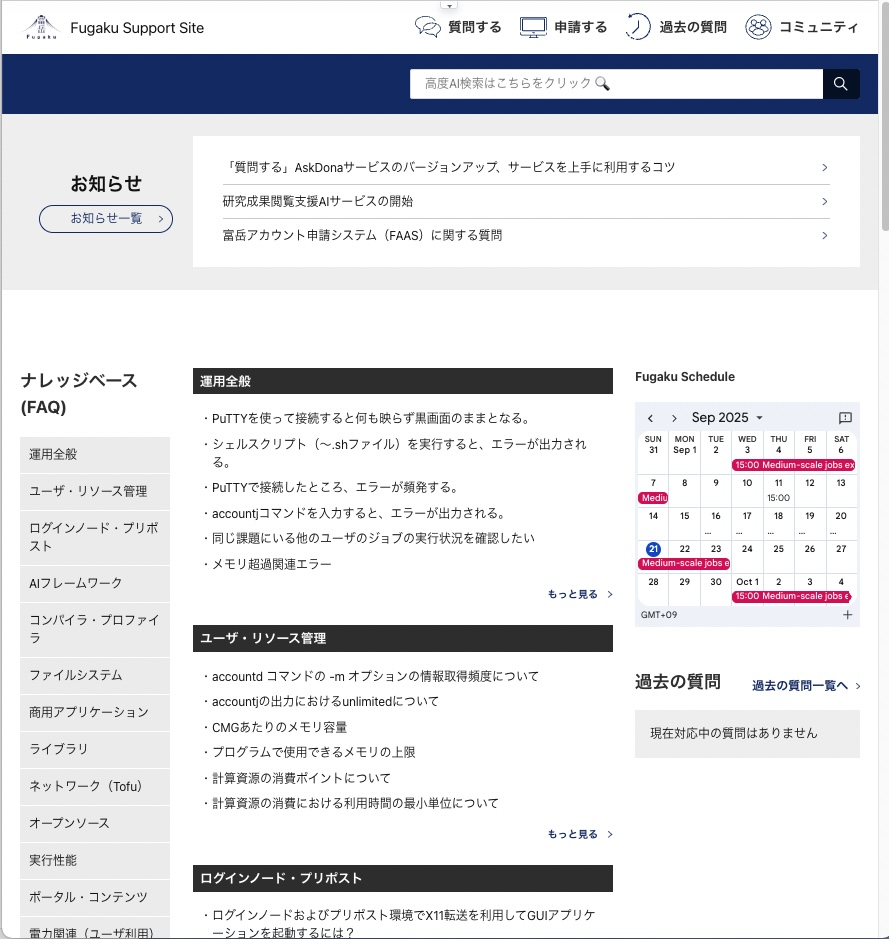
\includegraphics[width=\textwidth]{figs/FugakuSupportSite-Top.jpg}
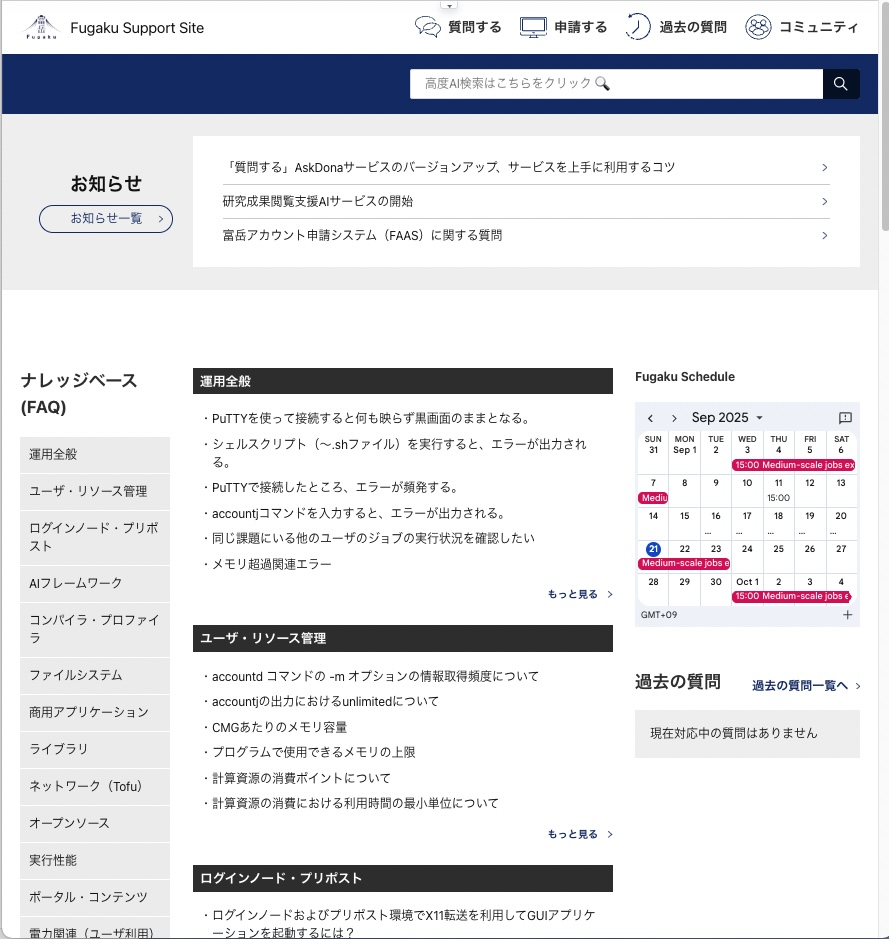
\includegraphics[width=8.5cm]{figs/FugakuSupportSite-Top.jpg}
\caption{富岳サポートサイトのUI}
\label{fig:FugakuSupportSite-Top.jpg}
\end{figure}



\subsection{「富岳サポートサイト」への生成AI応用サービスの導入}

「富岳サポートサイト」でのFAQ記事を充実させてユーザへ利便性の高い情報を提供するという手法は妥当な手段であったと考えられるものの、FAQ記事数が300を超える様になると、多数の記事の中から自分にとって有用な情報にたどり着くことが容易とは言えない状況となってきた。
各FAQ記事をカテゴリごとに分類して検索が容易となる様なレイアウトを採用したり、記事の件名から本文内容を想起し易いように記述するなど、運用側での努力継続されているが、有用なFAQ記事により直接的にたどり着くための手法の検討が必要となった。

さらに根本的な課題として、ユーザが「富岳」を利用して目的とする計算ジョブを実行して成果を得るために、「富岳」の利用手引書・各種マニュアル・講習会資料・性能データ等の100冊以上のドキュメント類に含まれる数万ページ相当の膨大な情報源から自分が必要とする情報を探し当てて確認する作業が相当の負担となることであった。
この状況においては従来型のキーワード検索手法はユーザが意図する情報検索の手段としては不十分であることも指摘される。
例えば、ある技術的な事項が複数のマニュアルに記載されることもしばしばあるが、
それらの内容は同一の場合もあれば、用途に応じて焦点の当て方を変えた異なる説明方法となっていることもある。
さらには、調査したい事項そのものが概念として表現はできるが、具体的なキーワードとして想起できないという状況もしばしばある。

膨大な情報蓄積資源の中から、ユーザ自身にとって必要な情報を適切に得るための手段を提供すること、ひいてはユーザ自身による問題解決を促進することは「富岳」を運用するチームにとって重要な課題であった。

このような背景のもと、近年非常に進化が進んだ生成AIを応用した質問への自動回答および高度検索サービスを導入する検討を2023年度から開始した。
様々なアプローチがあり得たが、サービスを利用する対象者が「富岳」ユーザであり、彼らが必要とする技術的情報は全て上述したドキュメント群のいずれかに記載されていることがわかっているため、それらのドキュメントから容易にかつ正確に必要な情報を調査提示することが可能な技術と目される検索拡張生成(RAG:Retrieval Augmented Generation)フレームワークを提供する複数の生成AIサービス事業者と実現の可能性について検討を進めた。

事業者各社との概念検証の実施、入札による事業者の決定を経て、2024年度に「富岳サポートサイト」へ「AIチャット」機能および「高度AI検索」機能としてサービスの追加を実施した。



\section{生成AI AskDona}


「富岳サポートサイト」の生成AIサービスは株式会社GFLOPSが開発したAskDonaを中心技術として採用している。AskDonaはマルチエージェント型の検索拡張生成(RAG:Retrieval Augmented Generation)機能をGFLOPS社独自の技術で構成し、大規模言語モデルとしてはGPTを組み入れたサービスである。

ユーザは質問入力をテキストで行う。
これは「富岳サポートサイト」の主要なサービスが基本的にはテキストベースで行われていること、
および「富岳」のほとんどのユーザがプログラムのコーディングやスクリプト作成等を自身で行う
と考えられ、質問の入力や解答の提示もなじみが深いテキスト形式が自然であろうとの判断による。

質問を受け付けたAskDonaは、
入力された質問文を分析し(transformer処理)、質問文に関連が強いデータチャンクをRAGの知識データベース(ベクトルデータ)から検索・取り出し(retrieve処理)、回答を構成する関連情報を含んだ質問文を大規模言語モデル(LLM)へのクエリとして送出し(プロンプト送信)、LLMから得られた回答内容をユーザへの回答文として統合化(synthesize処理)した上で、チャットウインドウ上で表示する。
AskDonaのデータ処理フローの概念図を
図\ref{fig:AskDona-Dataflow-J.jpg}
に示す。

\begin{figure}[htbp]
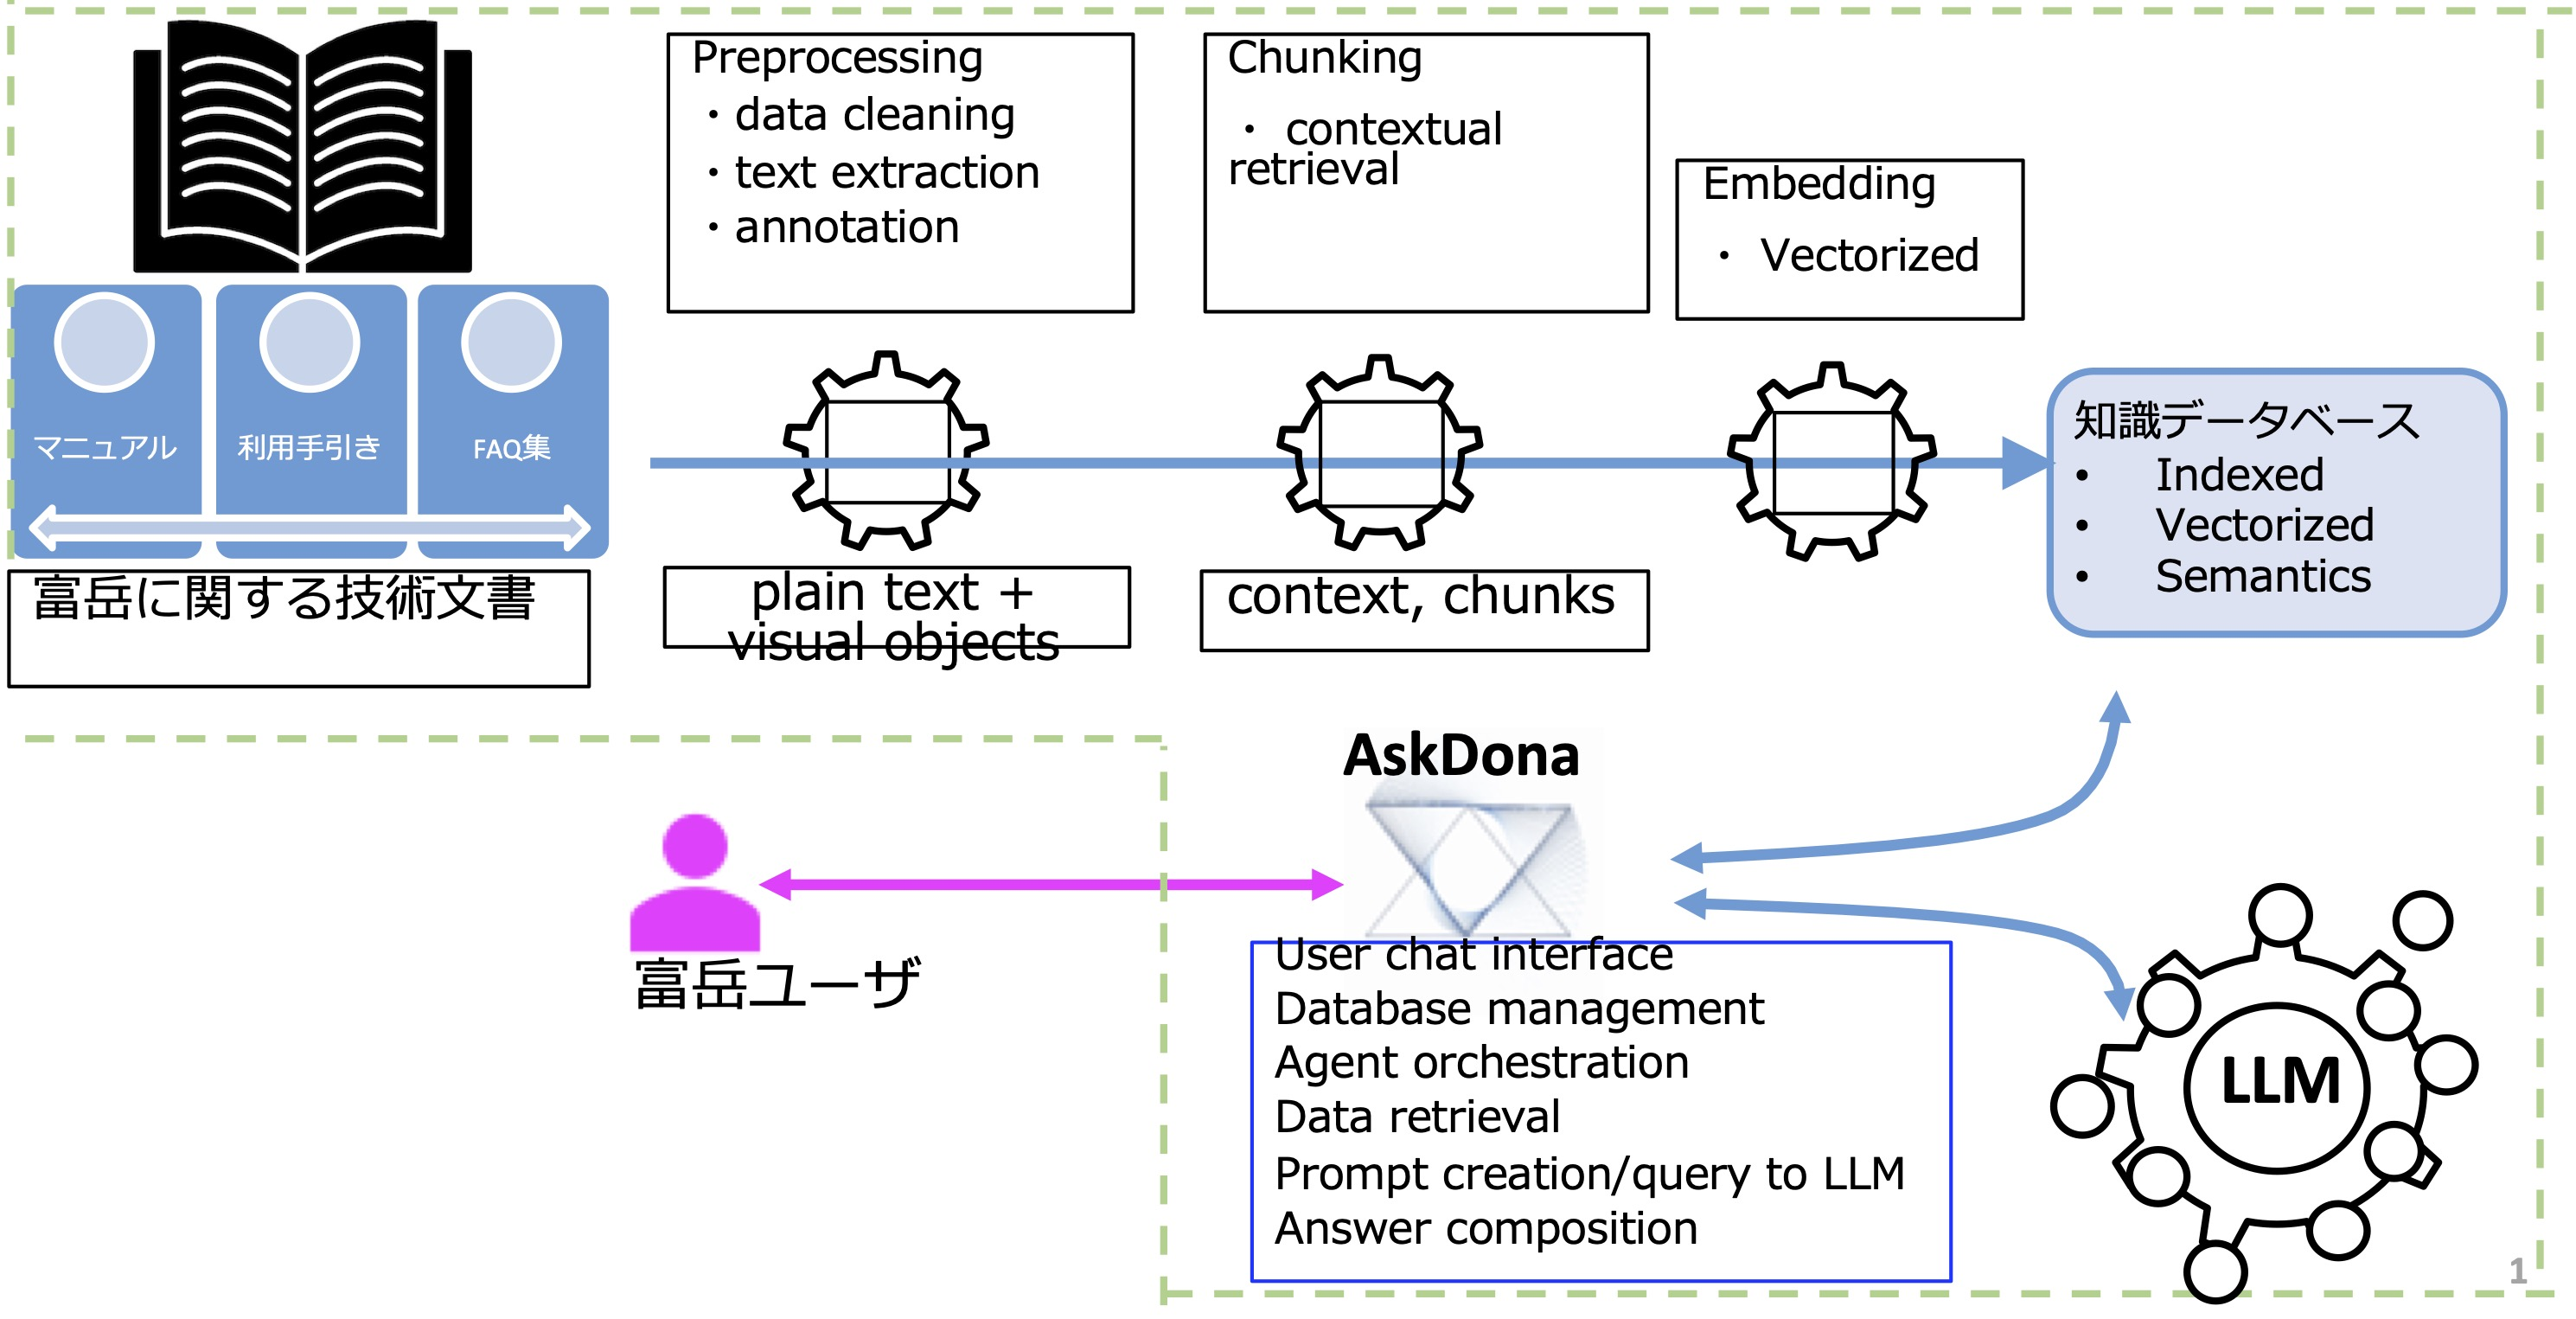
\includegraphics[width=8.5cm]{figs/AskDona-Dataflow-J.jpg}
\caption{AskDonaのデータフロー}
\label{fig:AskDona-Dataflow-J.jpg}
\end{figure}


トップメニュー上段の「質問する」をクリックすると生成AI AskDonaのチャットセッションが開始される。
AskDonaのユーザインタフェイスを図\ref{fig:AskDona-Chat-1.jpg}に示す。
チャットセッション下部に質問入力スペースがあり、調査の深度を選択可能となっている(Fast/Boost)。標準モード(Fast)での回答待ち時間は1分以下であり、通常は標準モードで適切な回答が得られることが多いが、より多角的な視点から多くの文書を分析して回答してほしい場合にはBoostモードを利用することができる。


\textcolor{red}{
Deep Research機能(多段階retrieval)について少し具体的に書けるだろうか?
発表日は12/3なので、それまでにはサービスを提供しているはず。\\
導入時のバージョン(dona-rag-1.0?)、現在のFastオプション、現在のBoostオプション, dona-rag-2.0, dona-rag-2.5(TBD?)についてまだ違いを十分に理解できていない。
}


\begin{figure}[htbp]
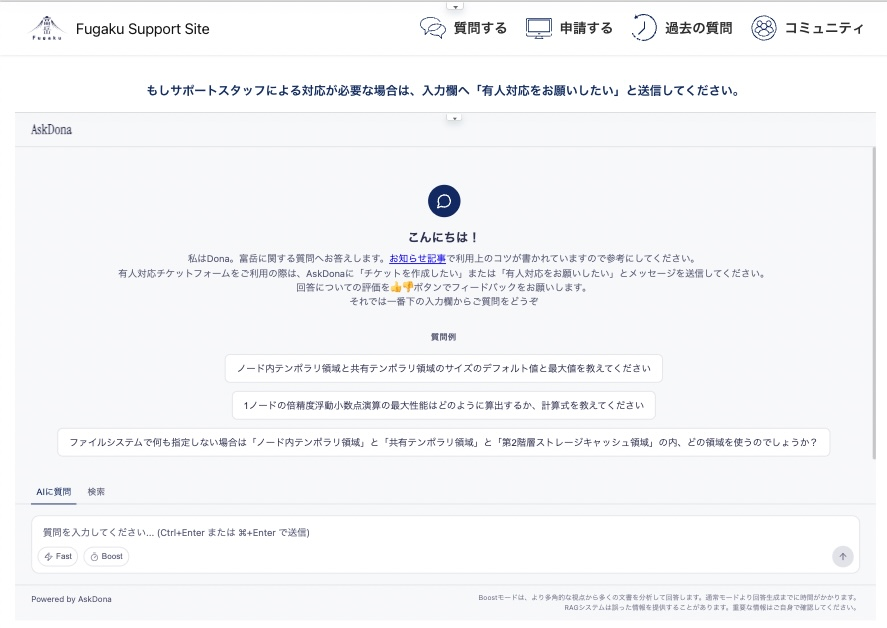
\includegraphics[width=8.5cm]{figs/AskDona-Chat-1.jpg}
\caption{生成AI応用サービスAskDonaのUI}
\label{fig:AskDona-Chat-1.jpg}
\end{figure}


以下に実際のユーザ質問とその解答例を示す。右上に反転色で質問文をエコー表示した後、回答文の作成が始まる。この例では30秒程度の待ち時間の後、まず回答の要約が表形式で表示され、続いて具体的な指定パラメタの説明と関連する注意事項、そして回答文で引用した参照元文書名がそのリンクとともに示されている。
改めて指摘するまでもなく、生成AIの回答が100\%正しい保証はない。
「富岳サポートサイト」の生成AIサービスが精度の高いRAG技術で構成されているとはいえ、ユーザ自身が参照元文書の該当箇所で
回答の正しさを確認することは、どのような生成AIを利用する場合でも共通する留意事項である。


\begin{figure}[htbp]
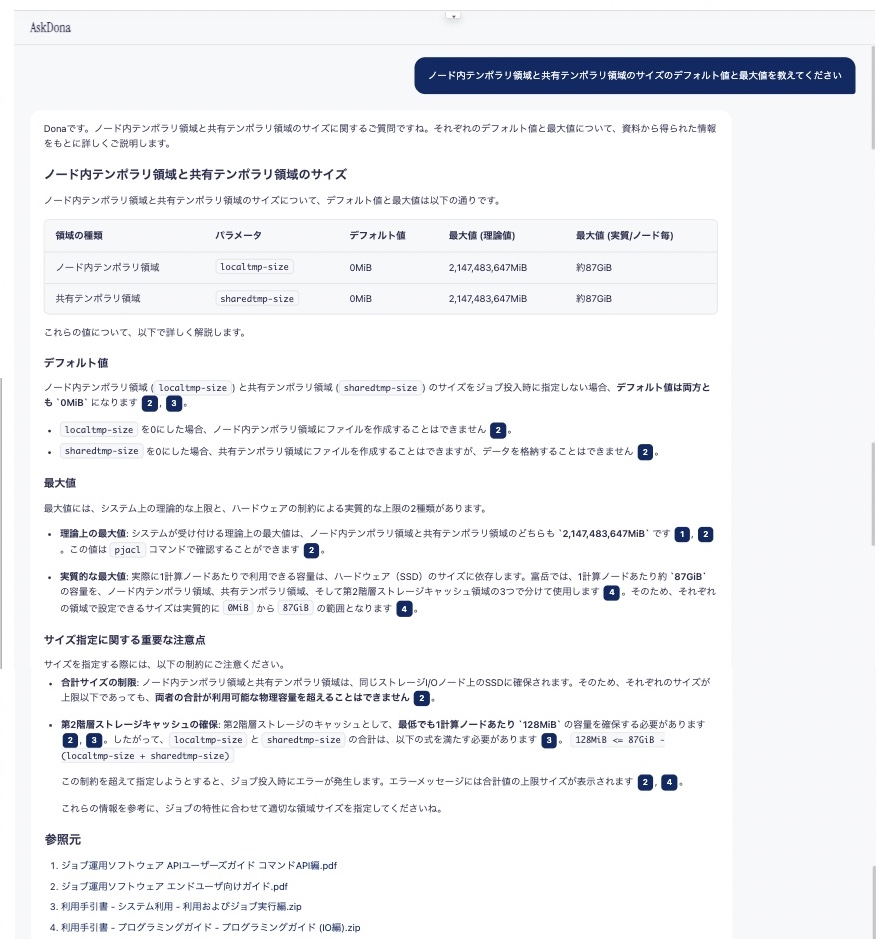
\includegraphics[width=8.5cm]{figs/AskDona-Answer.jpg}
\caption{AskDonaへの質問と回答の例}
\label{fig:AskDona-Answer.jpg}
\end{figure}

生成AI AskDonaによる質問回答サービスは 2024年度から始まり、当初はユーザが従来方式のチケット発行・有人対応サービスと、AskDonaによる自動回答サービスを選択できるメニューを提供していたが、半年間の経過観察を経て、全ての質問をAskDonaが最初に受け付けるメニューへ変更をおこなった。ユーザの質問へAskDonaがまず質問対応にあたるが、もし期待する回答がAskDonaから得られずに従来方式のチケット対応を希望する場合は、チャットセッションで「有人対応をお願いしたい」と入力することによりチケット発行メニューを呼び出すことができる。
このフローで発行されるチケットには AskDonaとのチャットセッション履歴を紐づける情報がサポートスタッフ向けに付加される。


R-CCSと株式会社GFLOPSが継続的に協働してきたことにより、AskDonaの回答精度は導入当初と比較して大きく向上している。
回答精度を向上するための具体的な施策として以下のようなことを行ってきた。

\begin{itemize}
	\item 元文書(特にマニュアル等のPDFファイル)からのノイズ除去と適切なラベリング
	\item 適切な元文書(特にFAQ記事)の充実化と知識データベースの更新
	\item retrieval手法の更新
	\item 適切な回答を得るためのシステムプロンプトの改良
	\item より高機能なLLMの採用
	\item 回答内容に満足・不満足が示されたチャットセッションを検知するツールの充実
\end{itemize}


\section{生成AI導入の効果}

\begin{itemize}

		\item 質問チケット数の推移
		\item ユーザのGood/Bad評価
		\item ユーザの質問内容の高度化
\end{itemize}
\textcolor{red}{
ちょっと息が切れた。このあたり中村さん手伝ってもらえますか?
}






\section{広範なHPCユーザに向けた展開:HPCI利用報告書の閲覧支援AIサービス}
前節までに説明したAskDona RAGによる生成AI技術が相当に効果的であると判明したことをうけて、
同技術を特定文書群の高度な調査支援ツールとして応用してはどうかとの意見が上がった。
具体的には革新的ハイパフォーマンス・コンピューティング・インフラ(HPCI)が提供する国内大学・研究機関のHPCシステムを課題利用した成果の報告書がHPCI研究成果ページに登録・公開されているが、これらを全て知識データベース化して、AskDonaを用いることにより様々な角度からの検索・比較・調査が可能となるサービスを立ち上げることである。
AskDonaの技術責任者と協議の上、そのプロジェクトに着手した。
2012年度から今年度までの利用報告書を全て知識データベース化する作業にとりかかり、1ヶ月程度の作業期間でデータベースの構築が完了した。
「富岳サポートサイト」において既にAskDonaのサービス環境を様々な改良を含めて実装済みである事から、「富岳サポートサイト」と同じZendesk基盤の上に「研究成果閲覧支援サービス」のページを設けた。
現時点でサービス立ち上げは完了し、HPCIのホームページから「HPCI研究成果」タグを辿れば、「富岳」ユーザに限らず全てのHPCユーザがアクセス・利用可能となっている。
「研究成果閲覧支援サービス」は興味ある課題の検索・報告書内容の論点整理・比較などの作業を自動的に行うことが可能なサービスであり、ユーザが課題に取り組む際に過去の研究事例を効率よく調べ上げるためのツールとしての利用が期待される。

「研究成果閲覧支援サービス」ページを開くと参考となりそうな質問例や必要に応じて選択できる絞り込みフィルターなどが準備されており、ユーザはこのサービスから得られる情報の期待感を持つことができる。

質問例から最初の一件をピックアップしてサービスを求めた実際の出力回答を一部抜粋して
図\ref{fig: AHPCI-covid19.jpg}に示す。

「新型コロナに関するテーマでの研究課題をリストアップして、課題の概要と、使用した計算資源を表にまとめてください。」

\begin{figure}[htbp]
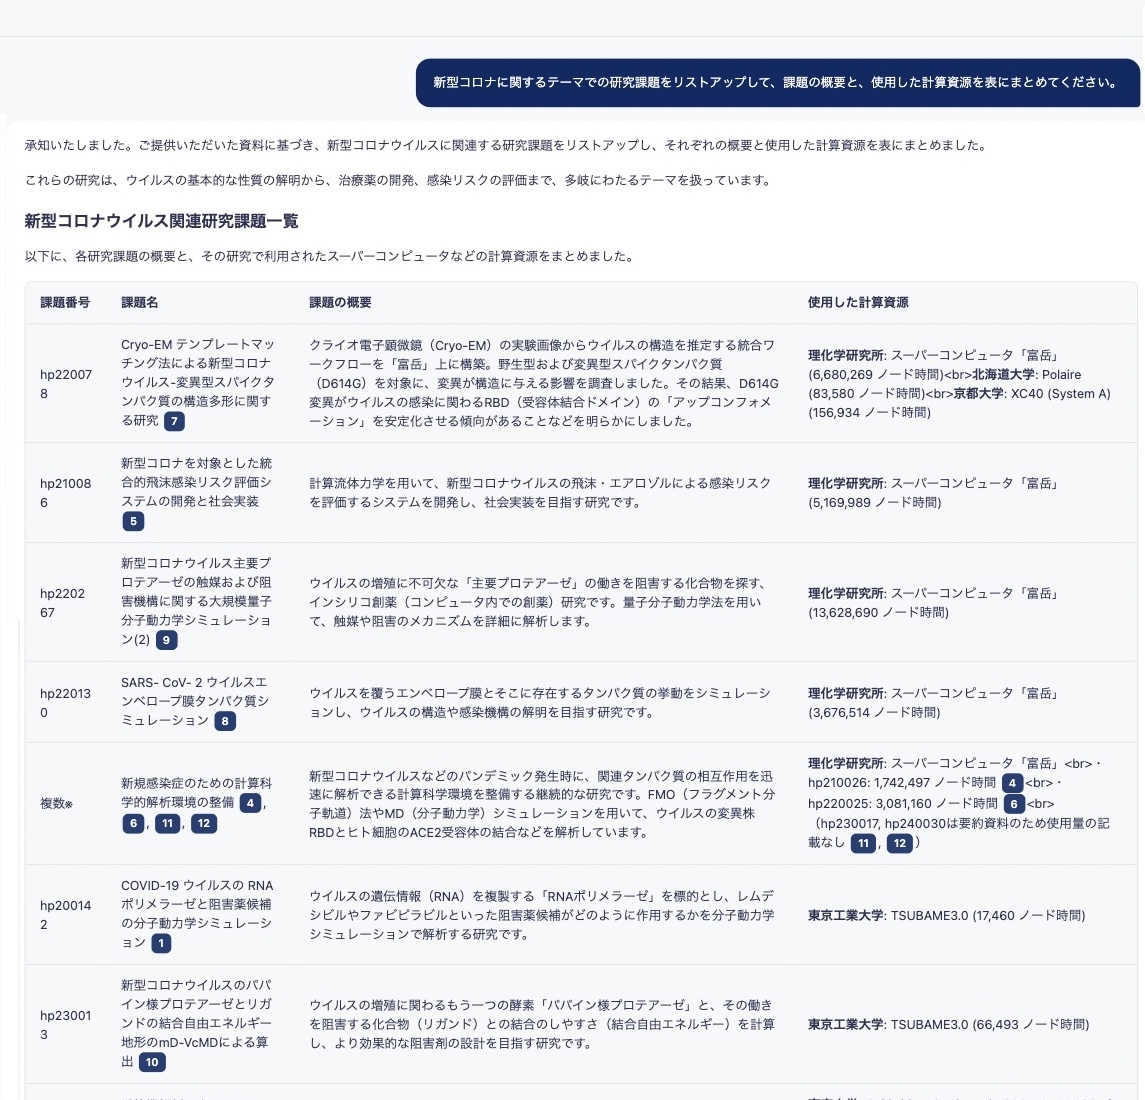
\includegraphics[width=8.5cm]{figs/HPCI-covid19.jpg}
\caption{研究成果閲覧支援サービスへの質問と回答の例}
\label{fig:AHPCI-covid19.jpg}
\end{figure}



本稿が発表される大学ICT推進協議会2025年度年次大会の会期までには、HPCI利用報告書に加えて、
JHPCN成果報告書も知識データベース化を完了する計画である。



\section{まとめと今後の展望}
「富岳サポートサイト」へ生成AIによるサービスを追加するにあたって、概念実証プロセスの詳細は割愛したが、最終的に決定された事業者が著しいペースで進むAI技術分野の進化に伴って様々な機能強化・改善要望に機動的に対応協力したことは、本サービスが定着する上での重要なポイントであった。


%参考文献
\begin{thebibliography}{99}
	\bibitem{refjournal} 雑誌の場合:著者名、タイトル、雑誌名 巻、号、ページ、発行年.
	\bibitem{refbook} 書籍の場合:著者名、書名、参照ページ、発行所、発行年.
\end{thebibliography}

\end{document}
